\section{Application Programming Interface}

Für jede Stufe der Pipeline existiert ein Plug-in, bestehend aus einer \textit{Facade-Klasse} und einer \textit{Settings-Klasse}. Erstere stellt diverse statische  Methoden zur Berechnung und zum Serialisieren der jeweiligen Ergebnisse bereit.
Letztere erbt von der Klasse \texttt{BaseSettings} (vgl. Abbildung \ref{fig:settings_common}) oder einer der Subklassen (siehe Abschnitt \ref{sec:matching_engine} - \ref{sec:patch_derivation_and_application}) und dient der Konfiguration der jeweiligen Komponente.

\class{org.sidiff.common.settings}{BaseSettings}{AbstractSettings}{
\begin{figure}[!h]
\centering
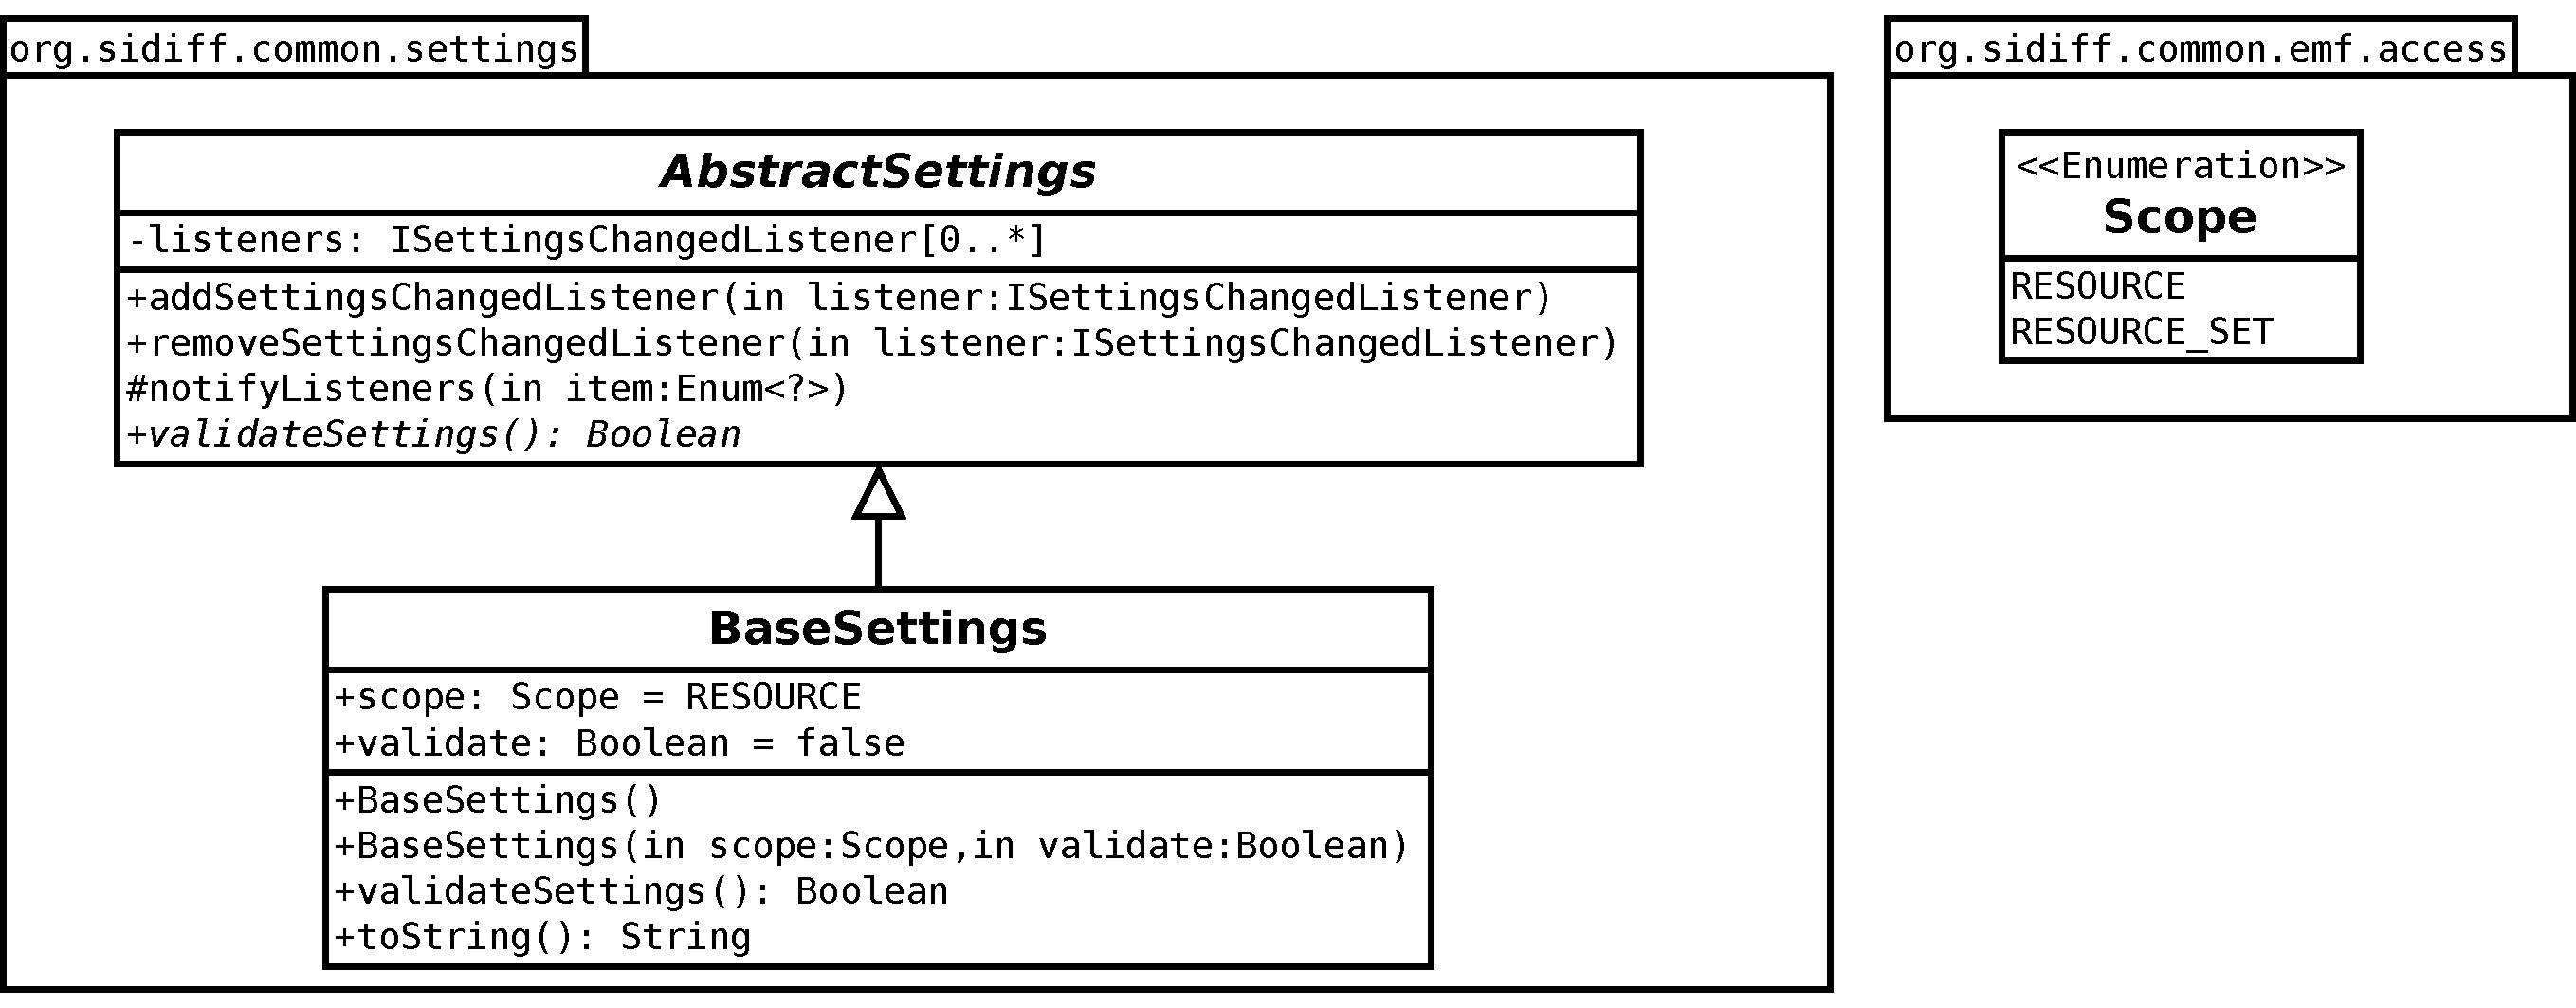
\includegraphics[width=0.75\textwidth]{images/api/settings_common.pdf}
\caption{Base Settings}
\label{fig:settings_common}
\end{figure}

Die Klasse \texttt{AbstractSettings} hält eine Liste von \texttt{ISettings\-Changed\-Listener}, mit deren Hilfe auf Änderungen einzelner Konfigurationsparameter reagiert werden kann. So kann die Belegung einzelner Parameter beispielsweise weitere Konfigurationsparameter aktivieren. Zusätzlich definiert die Klasse die Methode \texttt{validate\-Settings()}, um die Konfiguration zu validieren. Diese Methode muss von der jeweiligen Unterklasse implementiert bzw. überschrieben werden.\\
Die Klasse \texttt{BaseSettings} erbt von \texttt{AbstractSettings} und besitzt die beiden Konfigurationsparameter \texttt{scope} und \texttt{validate}. Ersterer legt fest, ob die folgenden Berechnungen auf Basis einer einzelnen Ressource (\texttt{Scope.RESOURCE}) oder einer Menge verbundener Ressourcen (\texttt{Scope.RESOURCE\_SET}) erfolgen. Über den Konfigurationsparameter \texttt{validate} kann festgelegt werden, ob die Eingabemodelle vor den folgenden Berechnungen validiert werden sollen.
}

\subsection{Matching Engine (org.sidiff.matching.api)}\label{sec:matching_engine}

\class{org.sidiff.matching.api}{MatchingFacade}{none}{
\begin{figure}[!h]
\centering
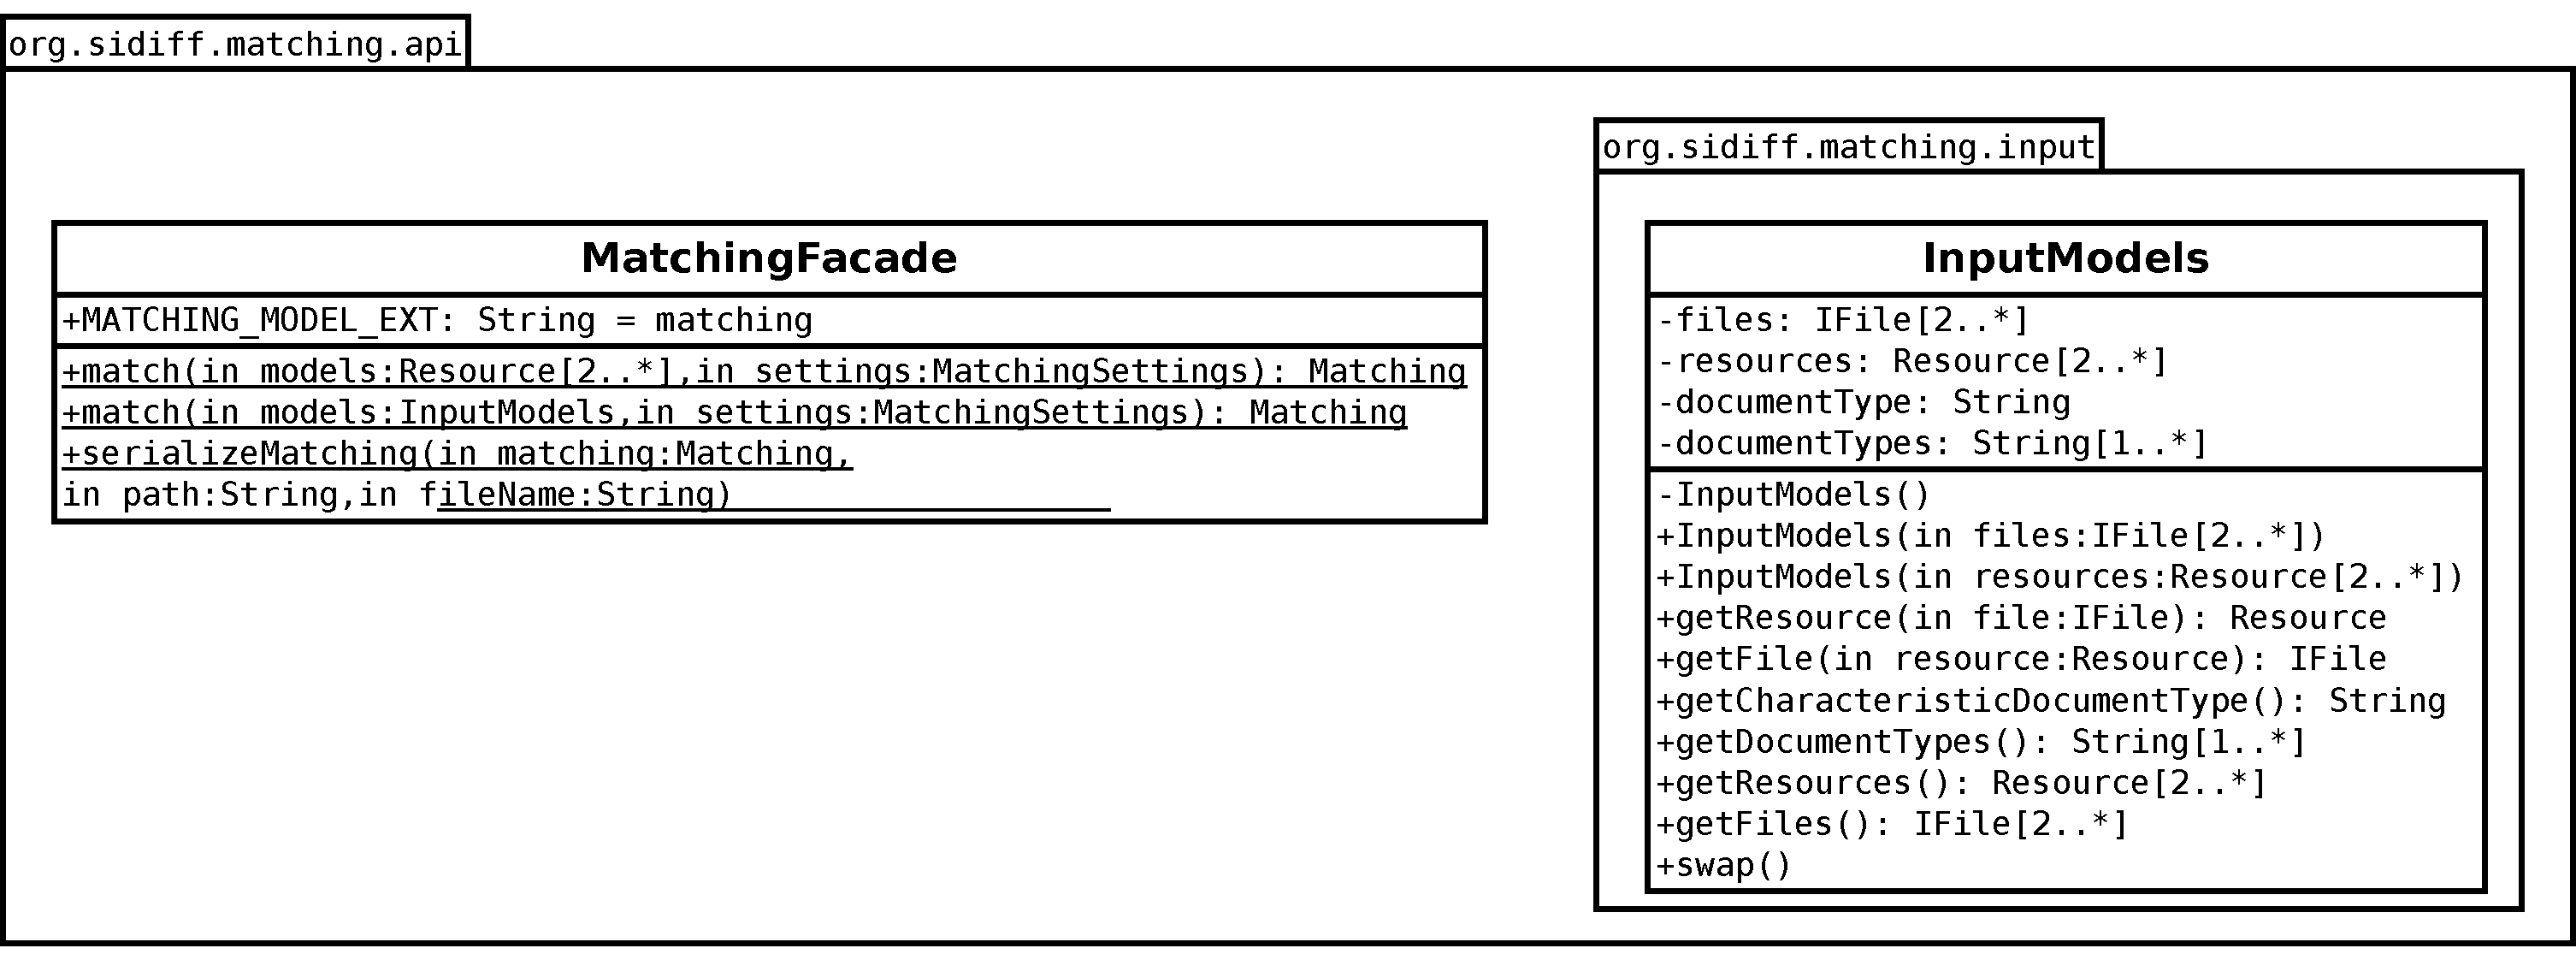
\includegraphics[width=0.75\textwidth]{images/api/facade_matching.pdf}
\caption{Matching Facade}
\label{fig:facade_matching}
\end{figure}

Die Klasse \texttt{MatchingFacade} stellt Methoden zur Verfügung, um Korrespondenzen zwischen mehreren Modellen zu berechnen (siehe Abbildung \ref{fig:facade_matching}: \texttt{match(...)}) und zu serialisieren (siehe Abbildung \ref{fig:facade_matching}: \texttt{serializeMatching(Matching matching, String path, String fileName)}). Anstatt der Methode \texttt{match()} eine Menge von Ressourcen vom Typ \texttt{org"".eclipse"".emf"".ecore"".resource"".Resource} zu übergeben, können diese auch in Form eines Objekts vom Typ \texttt{InputModels} übergeben werden. Diese Klasse ermöglicht den Zugriff auf die Ressourcen unter Verwendung von Ressourcen vom Typ \texttt{org"".eclipse"".core"".resources"".IFile}. Des Weiteren bietet die Klasse die Möglichkeit, die Reihenfolge der Eingabemodelle umzukehren.
}

\class{org.sidiff.matching.api.settings}{MatchingSettings}{BaseSettings}{
\begin{figure}[!h]
\centering
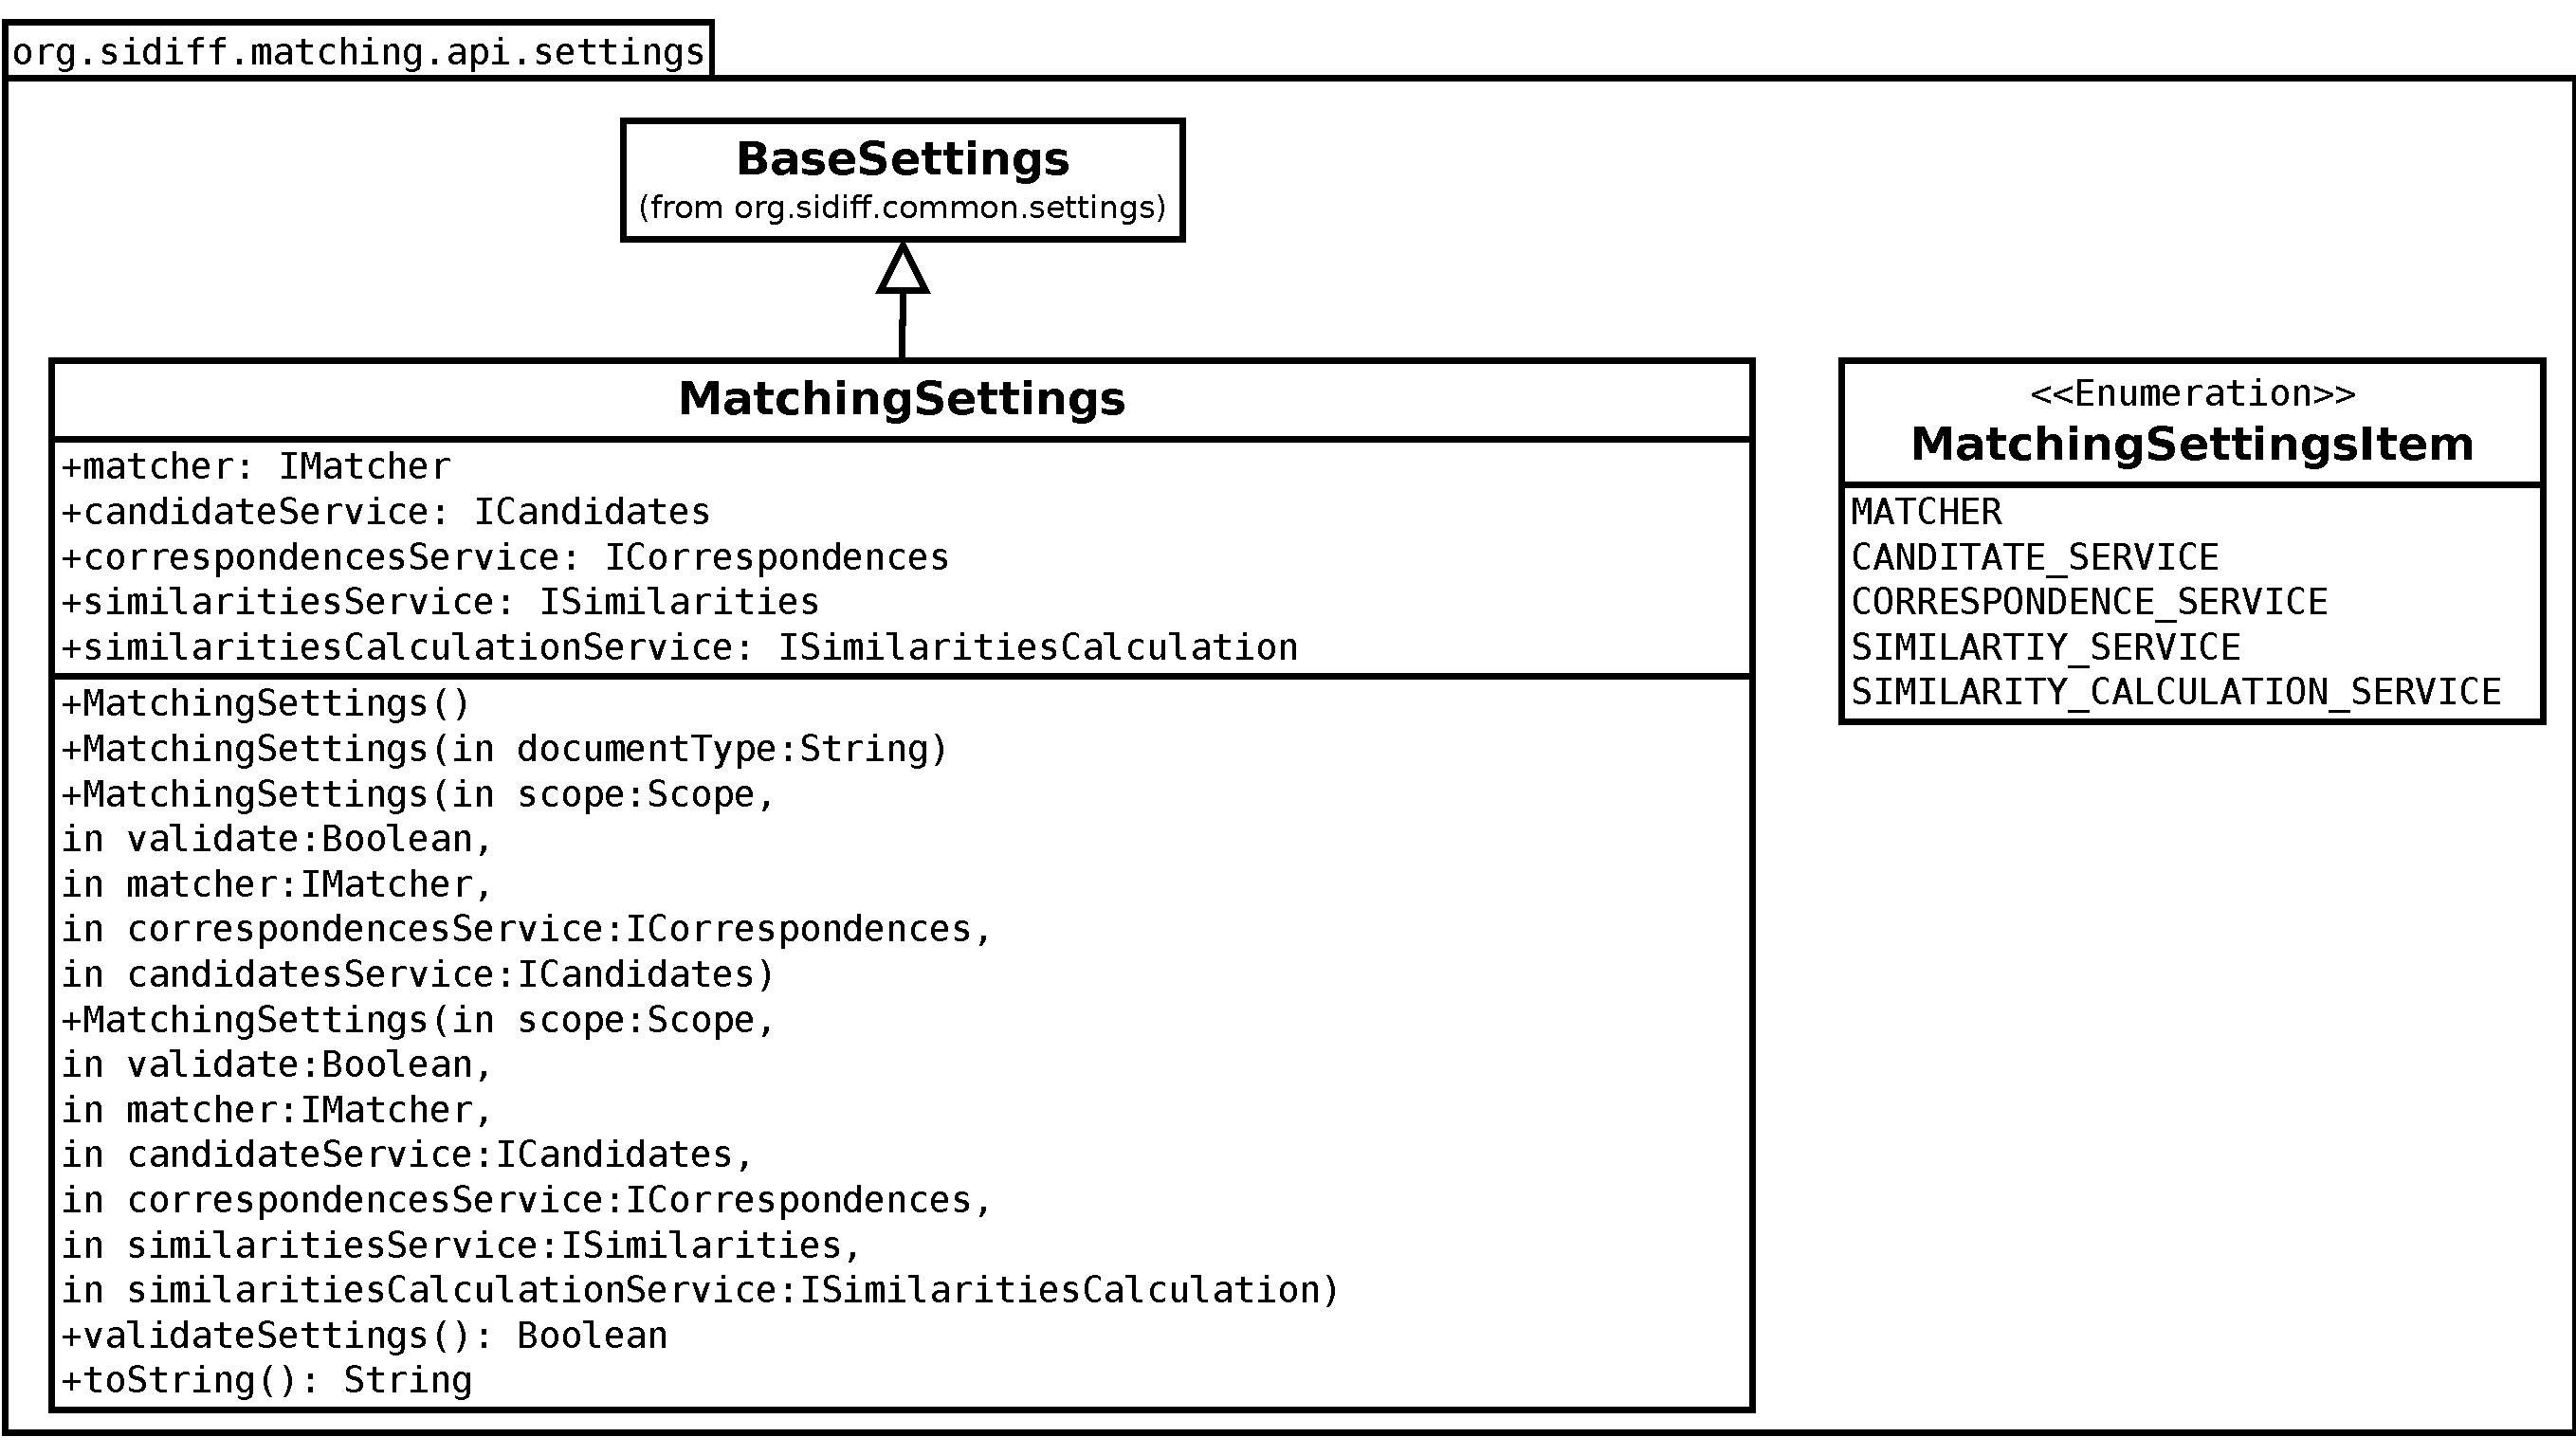
\includegraphics[width=0.75\textwidth]{images/api/settings_matching.pdf}
\caption{Matching Settings}
\label{fig:settings_matching}
\end{figure}
}

\subsection{Difference Derivator (org.sidiff.difference.technical.api)}\label{sec:difference_derivator}

\class{org.sidiff.difference.technical.api}{TechnicalDifferenceFacade}{MatchingFacade}
{
Die Klasse \textit{TechnicalDifferenceFacade} stellt Methoden zur Verfügung, um eine technische Differenz zwischen zwei Modellen zu berechnen und zu serialisieren.\\
}

\class{org.sidiff.difference.technical.api.settings}{DifferenceSettings}{MatchingSettings}{
\begin{figure}[!h]
\centering
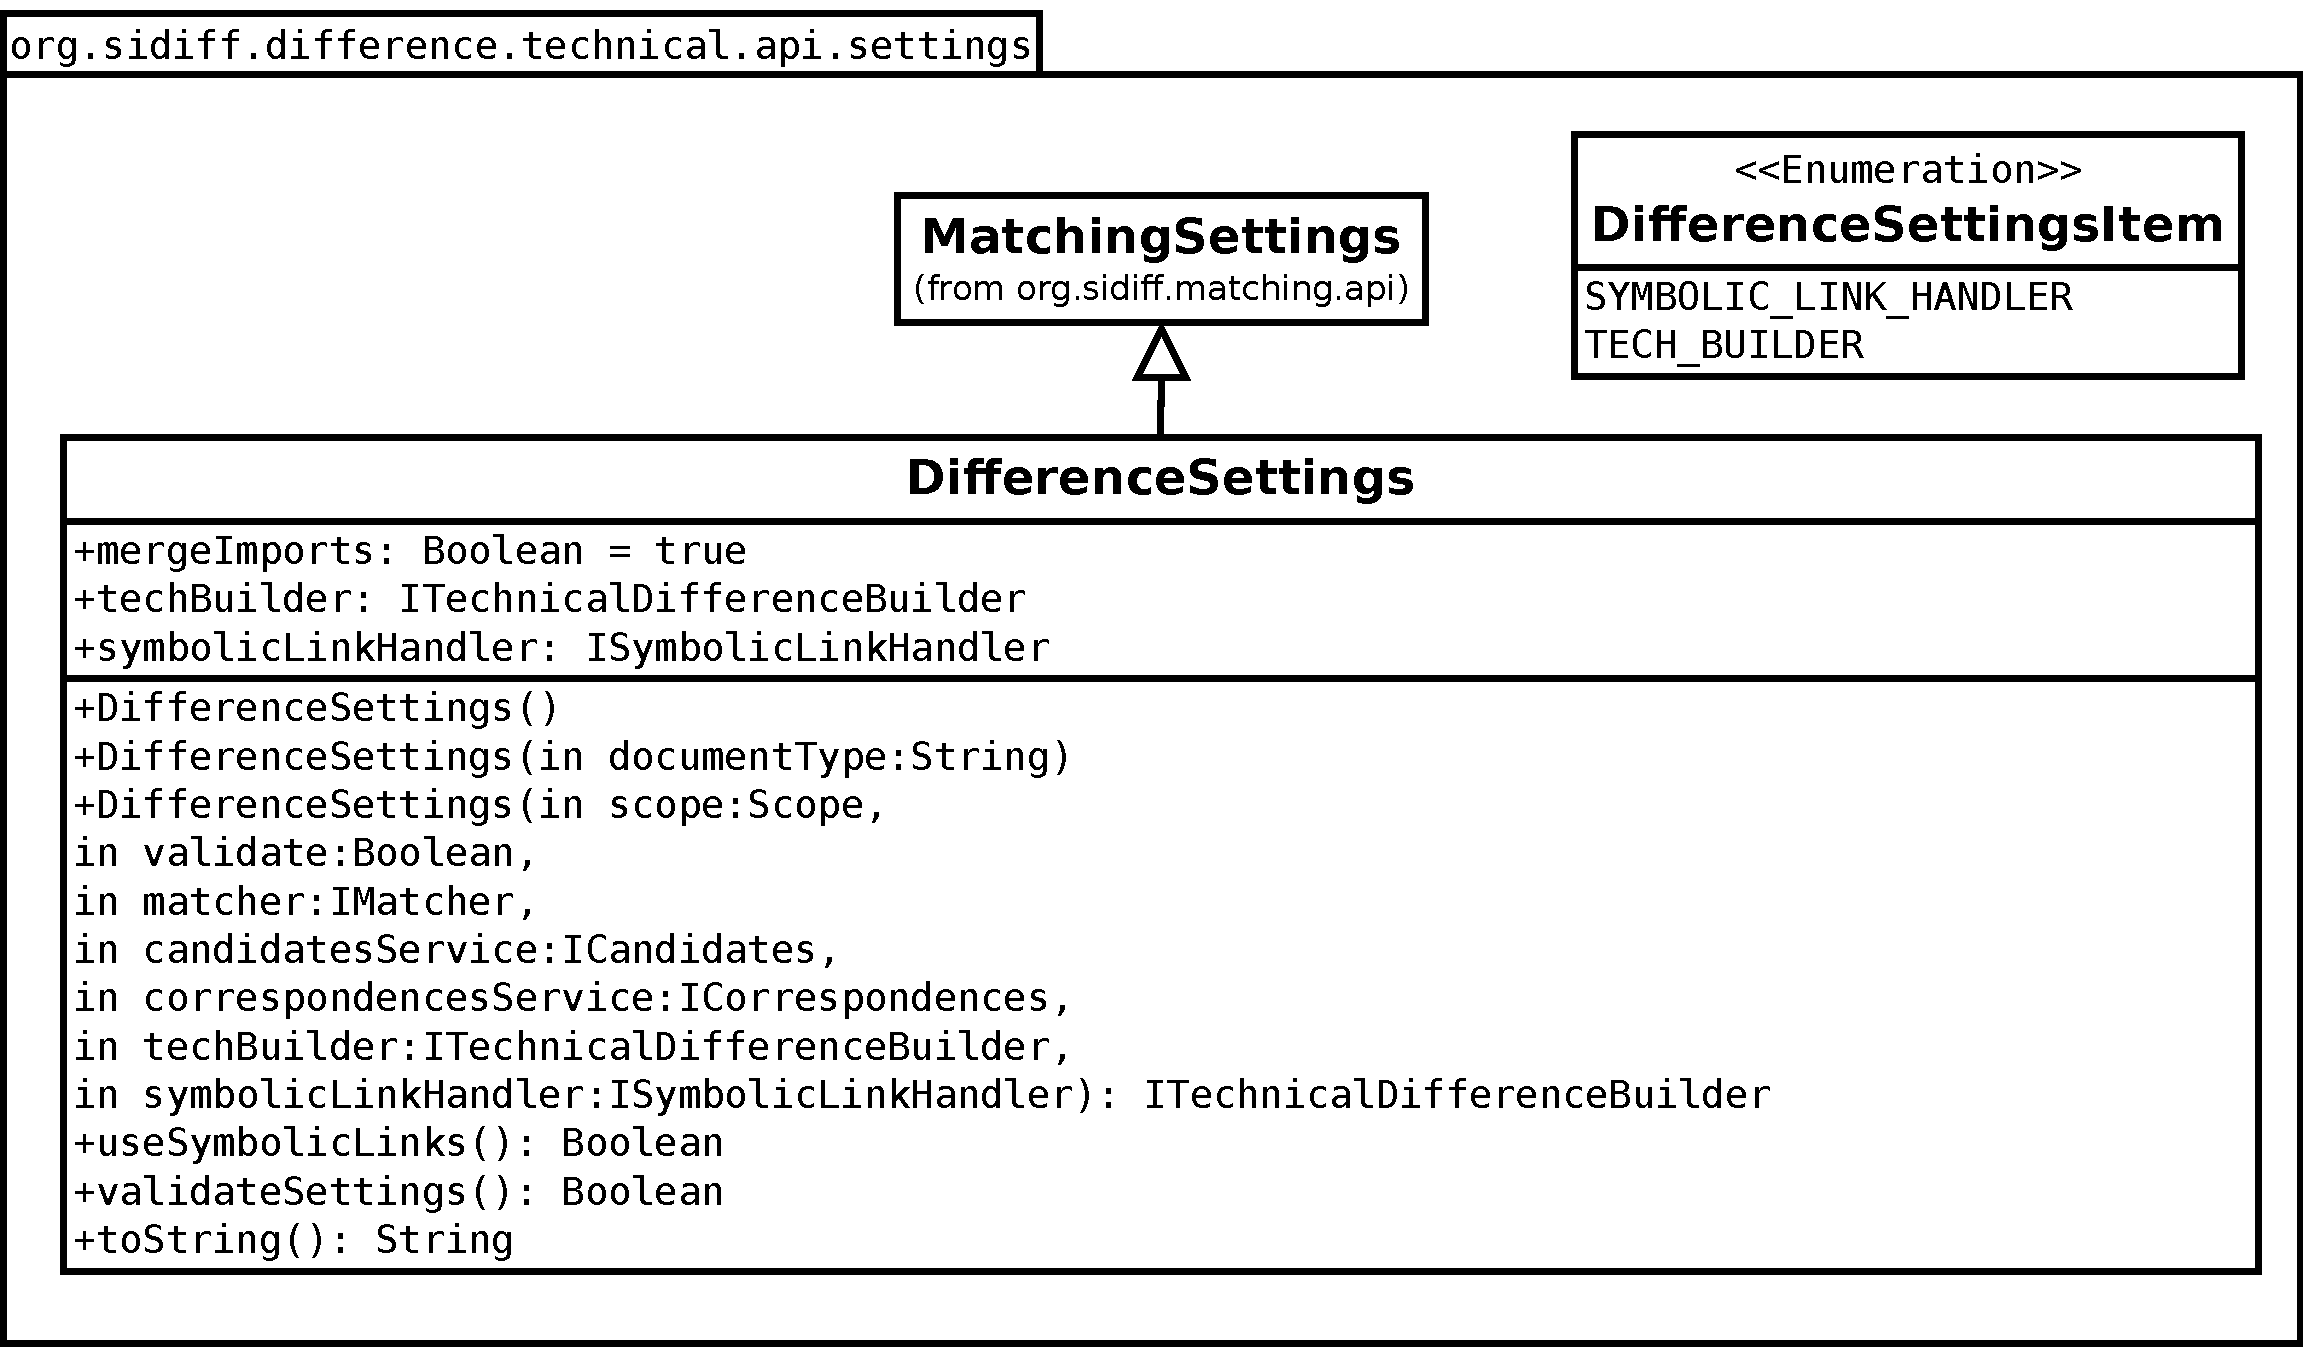
\includegraphics[width=0.75\textwidth]{images/api/settings_difference.pdf}
\caption{Difference Settings}
\label{fig:settings_difference}
\end{figure}
}

\subsection{LiftingEngine (org.sidiff.difference.lifting.api)}\label{sec:lifting_engine}

\class{org.sidiff.difference.lifting.api}{LiftingFacade}{TechnicalDifferenceFacade}{
Die Klasse \textit{LiftingFacade} stellt Methoden zur Verfügung, um eine technische Differenz semantisch zu lfiten und zu serialisieren.}

\class{org.sidiff.difference.asymmetric.api}{AsymmetricDiffFacade}{LiftingFacade}{
Die Klasse \textit{AsymmetricDiffFacade} stellt Methoden zur Verfügung, um eine geliftete, ausführbare, asymmetrische Differenz zu berechnen und zu serialisieren.}

\class{org.sidiff.difference.lifting.api.settings}{LiftingSettings}{DifferenceSettings}{
\begin{figure}[!h]
\centering
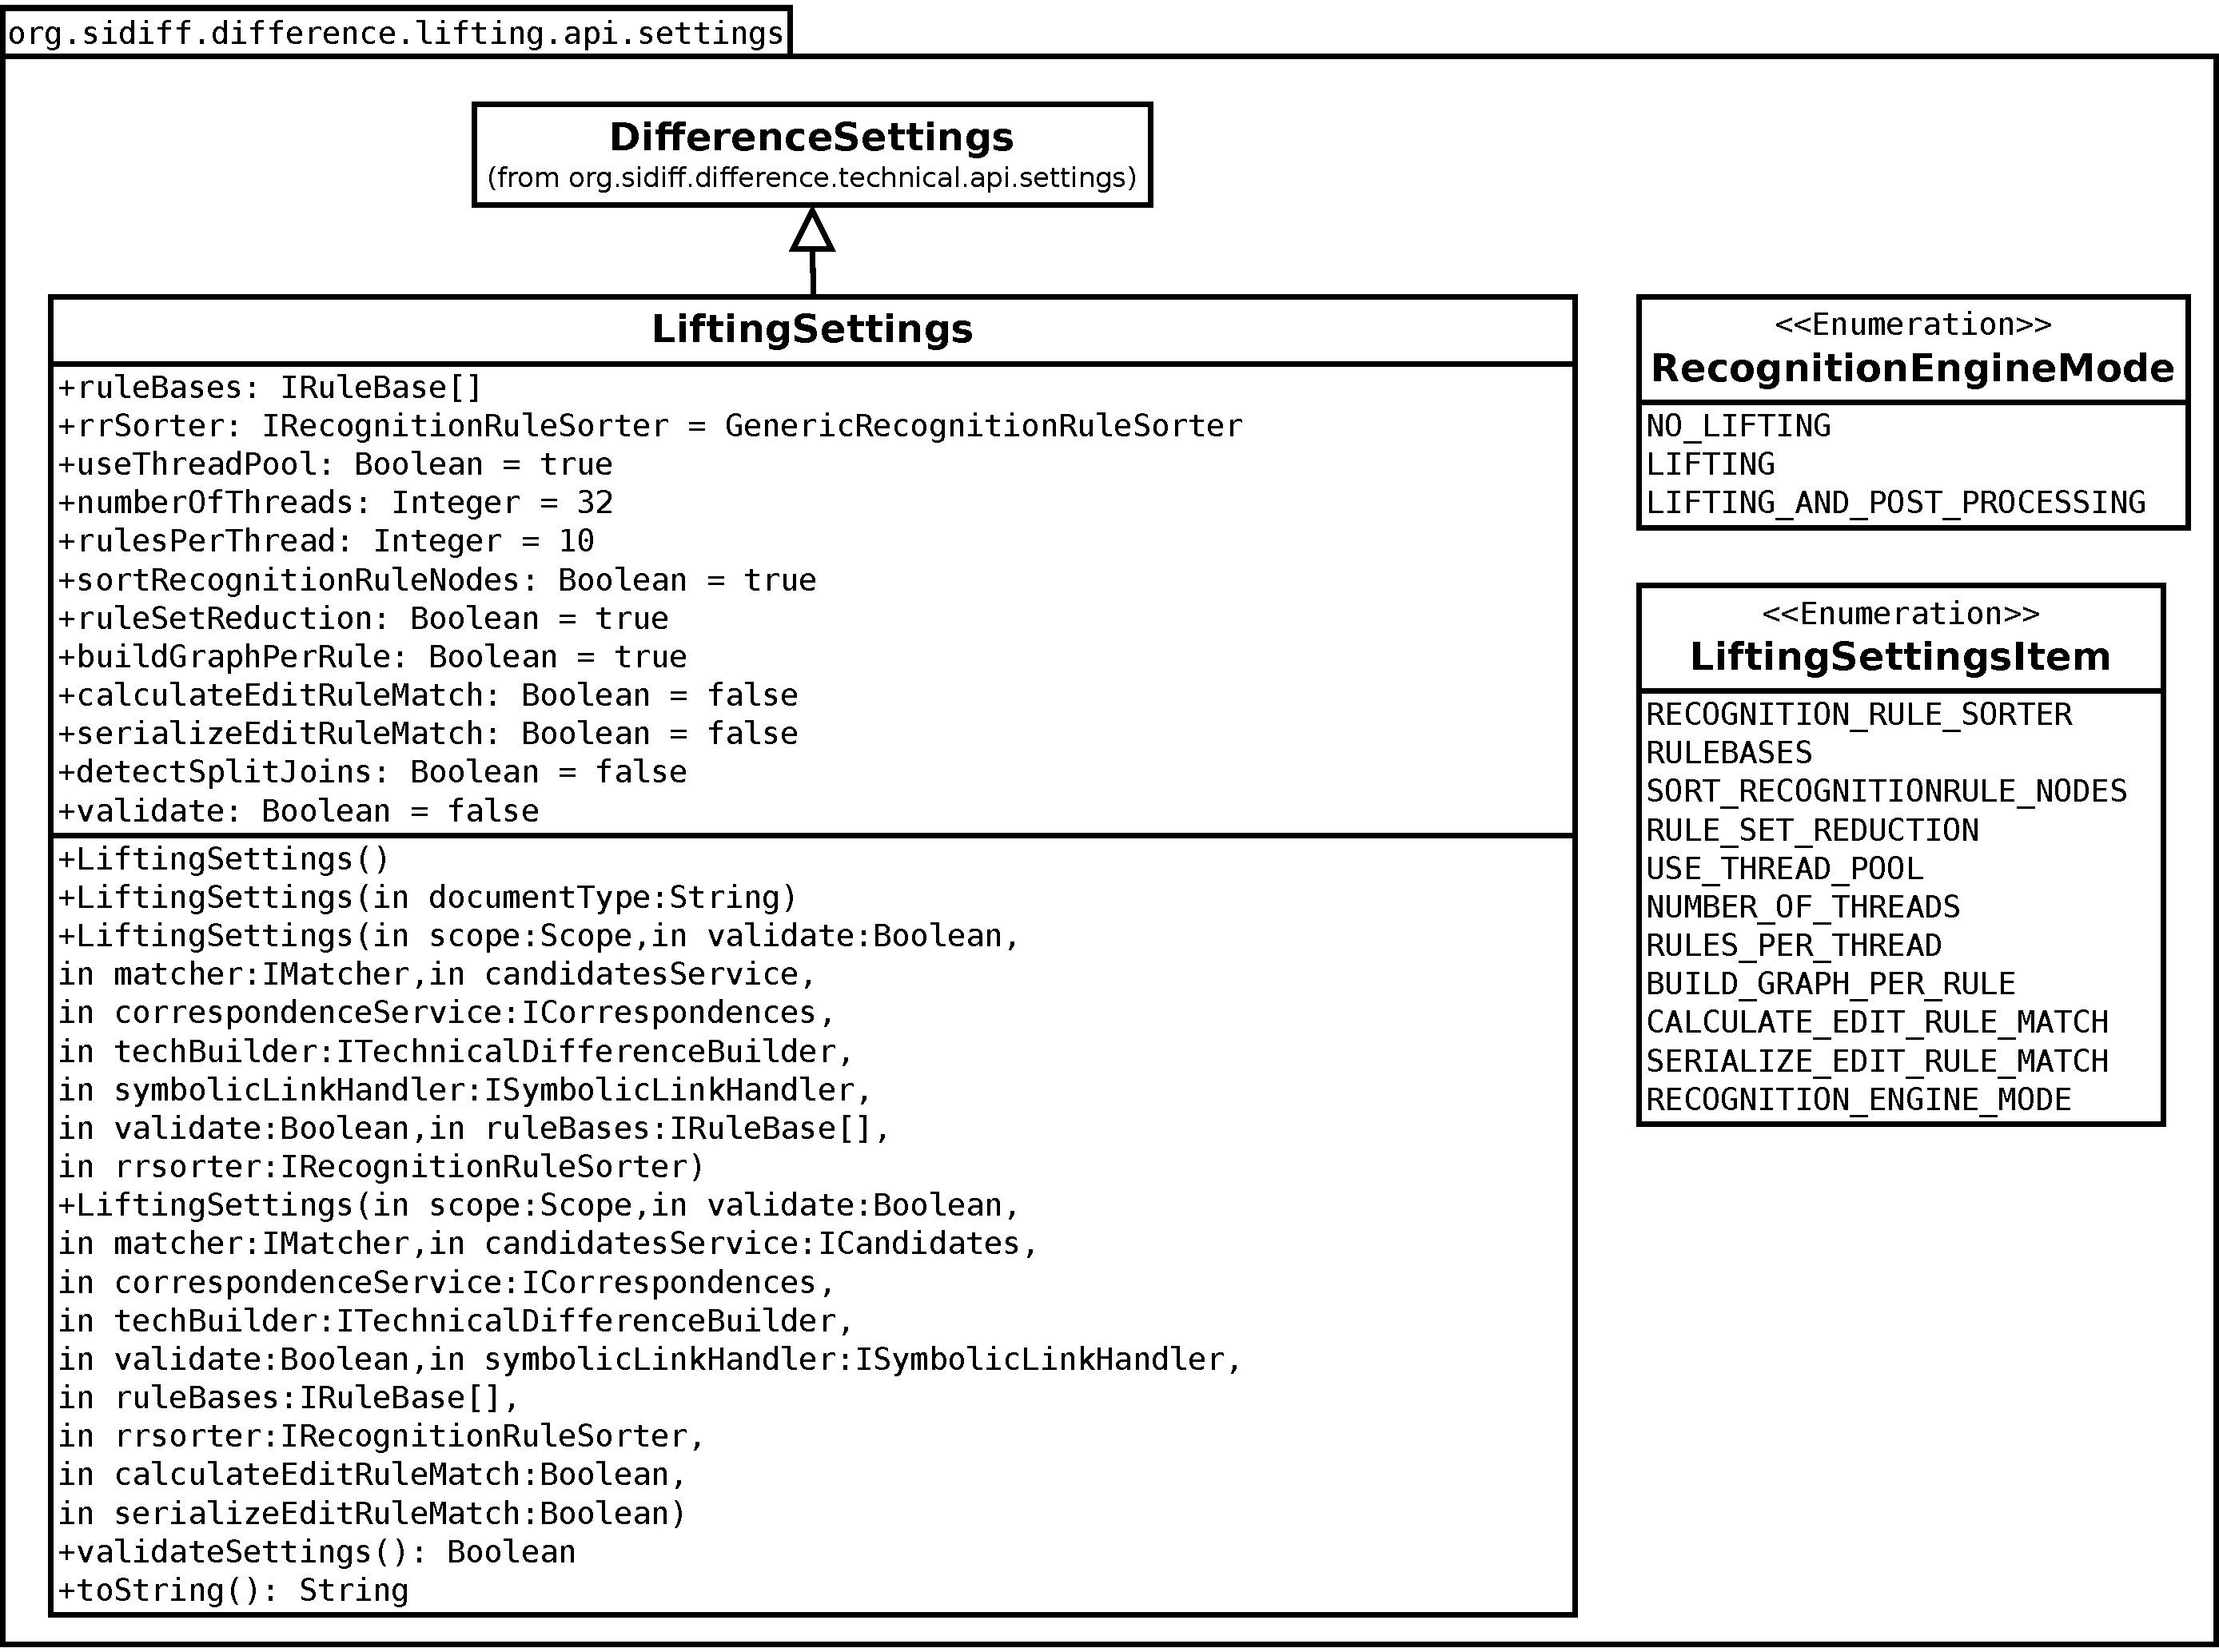
\includegraphics[width=0.75\textwidth]{images/api/settings_lifting.pdf}
\caption{Lifting Settings}
\label{fig:settings_lifting}
\end{figure}
}

\subsection{Patch Derivation and Application (org.sidiff.patching.api)}\label{sec:patch_derivation_and_application}